\documentclass{beamer}
  % Beamer settings
  \usetheme{CambridgeUS}
  \usecolortheme{seagull}
  \usefonttheme{professionalfonts}
  \usefonttheme{serif}

  % Packages and package settings
  \usepackage{fontspec}
    \setmainfont{Charis SIL}
  \usepackage{hyperref}
    \hypersetup{colorlinks=true,
                allcolors=blue}
  \usepackage[backend=biber, style=apa]{biblatex}
    \addbibresource{References.bib}
  \usepackage{graphicx}
    \graphicspath{{./figures/}}

  % Document information
  \author{Joshua McNeill}
  \date{4 February 2020}
  \title{Overview of Dubois \& Horvath (2003)}

\begin{document}
  \begin{frame}
    \titlepage
  \end{frame}

  \begin{frame}{Article}
    \fullcitebib{dubois_verbal_2003}
  \end{frame}

  \begin{frame}{Plan}
    \tableofcontents
  \end{frame}

  \AtBeginSection{
    \begin{frame}{Plan}
      \tableofcontents[currentsection]
    \end{frame}
  }

  \section{Introduction}
    \begin{frame}{Cajun Vernacular English (CVE)}
      \begin{definition}
        A variety ``spoken by French/Enlgish bilinguals and, to some extent, English monolinguals living in French-dominant rural areas of south Louisiana.''
      \end{definition}
      \begin{block}{An ethnolect?}
        ``We have in previous articles referred to \alert{Cajun} English as an \alert{ethnolect}, and in this article we have chosen to call it a \emph{vernacular} (after Gillian Sankoff’s suggestion at NWAV 29).
        The sets of key words found in many dictionary definitions for the word \emph{vernacular} are (1) originating, native, indigenous and (2) place, land, or country.
        What is attractive about the term vernacular is the focus on `originating in a place where it is used' because this succinctly captures the point we are trying to make about the origins of Cajun English.'' [bold mine]
      \end{block}
    \end{frame}

    \begin{frame}{Objective}
      \begin{block}{Determine the relationship of CVE to other languages/varieties}
        \begin{enumerate}
          \item Is it the result of French interference?
          \item Is it the result of the influence of Southern English?
          \item \emph{Is it the result of innovations from within the community?}
        \end{enumerate}
      \end{block}
    \end{frame}

    \begin{frame}{Variables}
      \begin{center}
        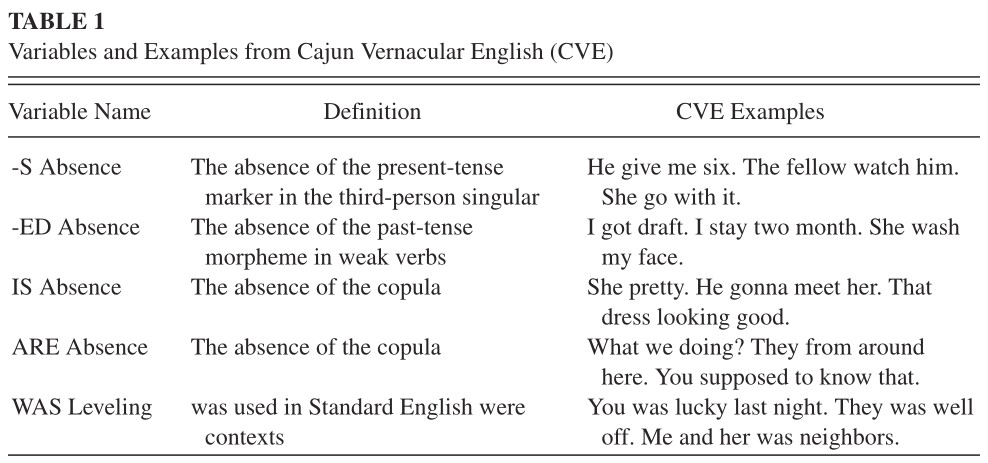
\includegraphics[scale=0.65]{variables.jpg}
      \end{center}
      \begin{block}{}
        Found in SE and AAE, but not expected at the same rates
      \end{block}
    \end{frame}

    \begin{frame}{Who are Cajuns?}
      \begin{block}{Implicitly}
        Rural south Louisianians who have some sort of French language heritage
      \end{block}
      \begin{block}{Explicitly}
        Cajun identity is associated with men who:
        \begin{itemize}
          \item fish, hunt, and partake in Cajun activities
        \end{itemize}
      \end{block}
    \end{frame}

  \section{Methodology}
    \begin{frame}{Sample and analysis}
      \begin{block}{NORMs mostly}
        16 young (b.~1960s) and old (b.~before 1930) men who
        \begin{itemize}
          \item speak or don't speak French,
          \item are or are not more educated, and
          \item who have lived in the same parish all their lives
        \end{itemize}
      \end{block}
      \begin{alertblock}{}
        Only men used non-standard features in their previous studies
      \end{alertblock}
      \begin{block}{Goldvarb analysis}
        i.e., Binomial regression
      \end{block}
    \end{frame}

  \section{Results}
    \begin{frame}{General}
      \begin{center}
        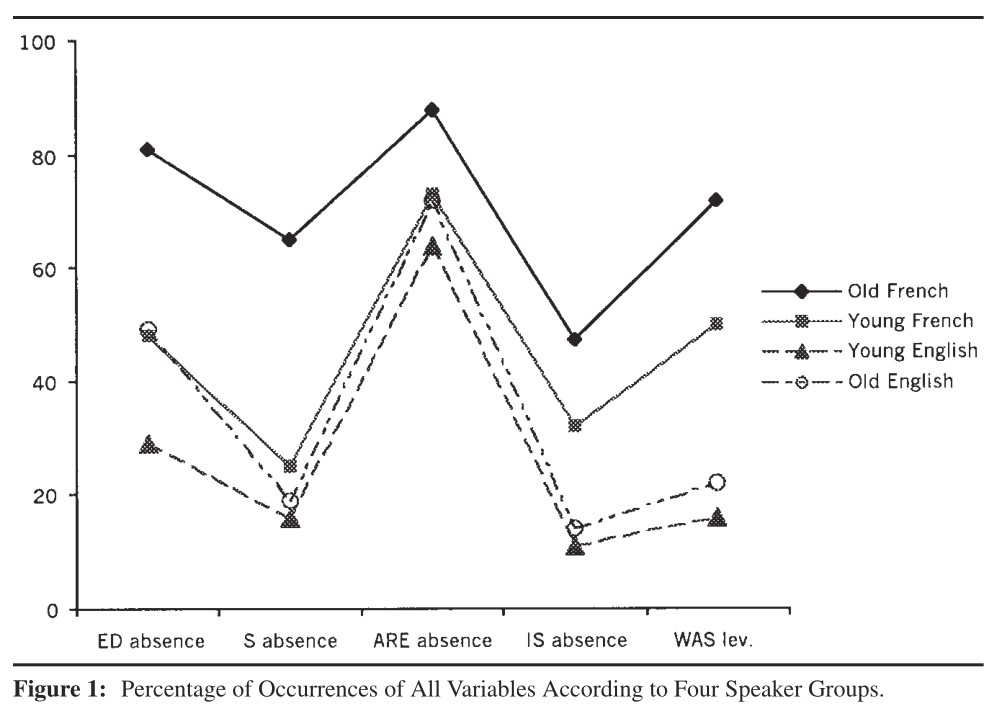
\includegraphics[scale=0.5]{general_results.jpg}
      \end{center}
    \end{frame}

    % \begin{frame}{General}
    %   \begin{block}{Education was statistically significant}
    %     \begin{itemize}
    %       \item More education, less non-standard
    %       \item Less education, more non-standard
    %     \end{itemize}
    %   \end{block}
    % \end{frame}

    \begin{frame}{\emph{-ed} Absence, not quite like the others}
      \begin{center}
        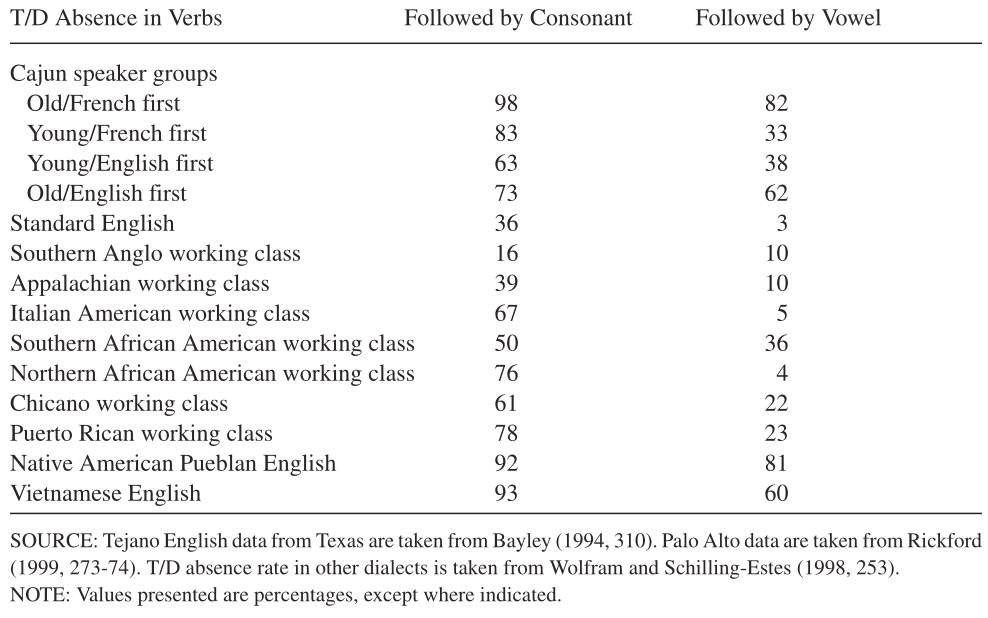
\includegraphics[scale=0.65]{ed_absence.jpg}
      \end{center}
      % \begin{block}{}
      %   \begin{itemize}
      %     \item Older speakers ressemble Native Americans and Vietnamese, younger no groups
      %     \item Younger speakers don't pattern well with any other group
      %   \end{itemize}
      % \end{block}
    \end{frame}

    \begin{frame}{\emph{are} Absence, high for loc and adj}
      \begin{center}
        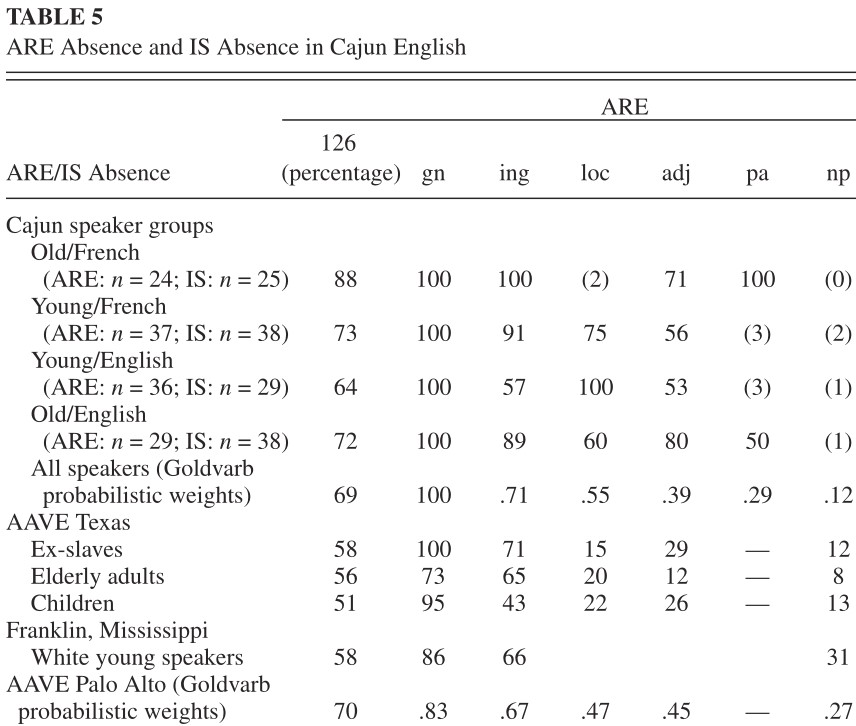
\includegraphics[scale=0.55]{are_absence.jpg}
      \end{center}
    \end{frame}

    \begin{frame}{\emph{was} Leveling}
      \begin{center}
        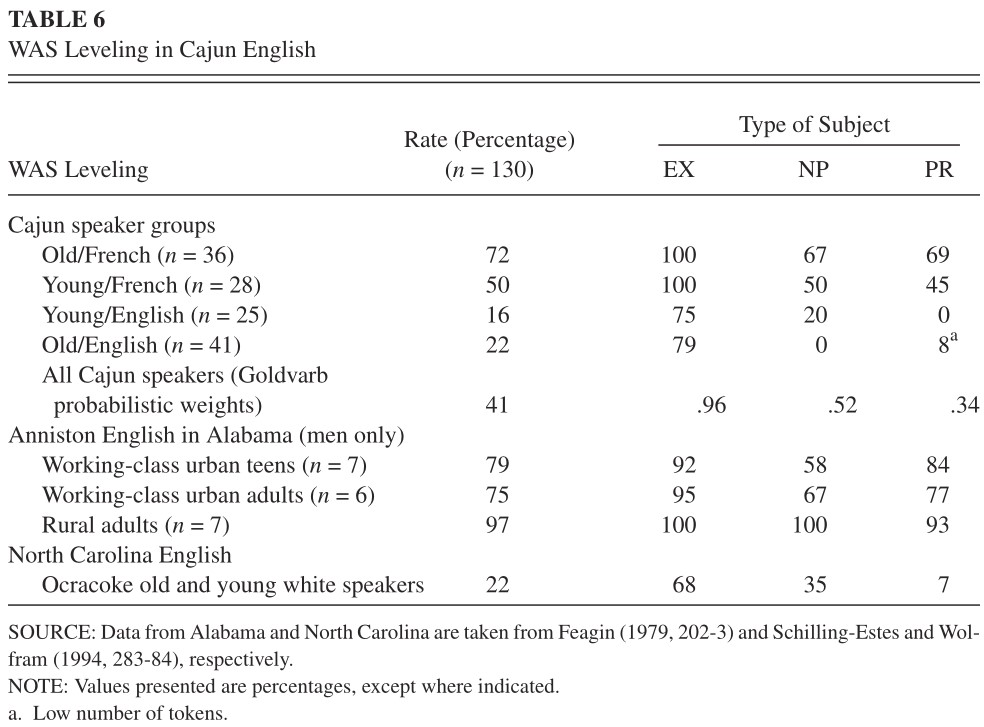
\includegraphics[scale=0.5]{was_leveling.jpg}
      \end{center}
    \end{frame}

    \begin{frame}{Final consonant deletion, a Cajun-specific variable}
      \begin{center}
        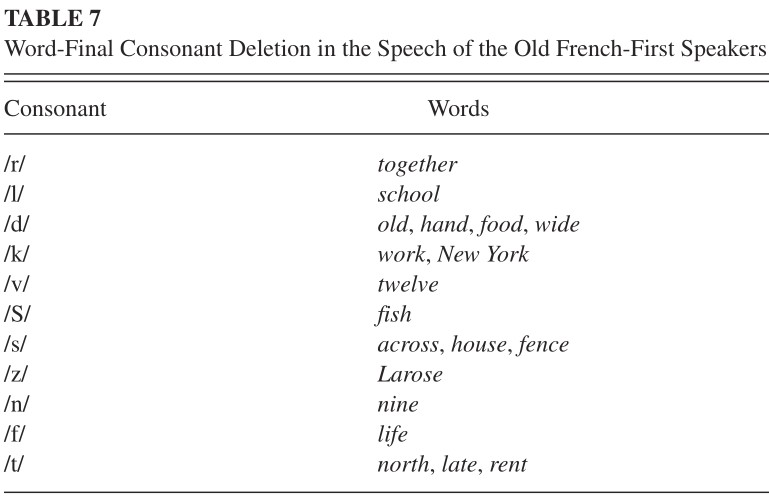
\includegraphics[scale=0.65]{final_deletion.jpg}
      \end{center}
    \end{frame}

  \section{Discussion}
    \begin{frame}{Southern English relationship}
      \begin{block}{}
        \begin{itemize}
          \item Early CVE cannot be derived from SE
          \item Later CVE influenced by greater access to SE from WWII on
        \end{itemize}
      \end{block}
    \end{frame}

    \begin{frame}{French relationship}
      % Interference would have disappeared after a generation
    \end{frame}
\end{document}
